\documentclass{beamer}
\usepackage[utf8]{inputenc}

\usetheme{Madrid}
\usecolortheme{default}
\usepackage{amsmath,amssymb,amsfonts,amsthm}
\usepackage{tkz-euclide}
\usepackage{listings}
\usepackage{adjustbox}
\usepackage{array}
\usepackage{tabularx}
\usepackage{gvv}
\usepackage{lmodern}
\usepackage{circuitikz}
\usepackage{tikz}
\usepackage{graphicx}

\setbeamertemplate{page number in head/foot}[totalframenumber]

\usepackage{tcolorbox}
\tcbuselibrary{minted,breakable,xparse,skins}



\definecolor{bg}{gray}{0.95}
\DeclareTCBListing{mintedbox}{O{}m!O{}}{%
  breakable=true,
  listing engine=minted,
  listing only,
  minted language=#2,
  minted style=default,
  minted options={%
    linenos,
    gobble=0,
    breaklines=true,
    breakafter=,,
    fontsize=\small,
    numbersep=8pt,
    #1},
  boxsep=0pt,
  left skip=0pt,
  right skip=0pt,
  left=25pt,
  right=0pt,
  top=3pt,
  bottom=3pt,
  arc=5pt,
  leftrule=0pt,
  rightrule=0pt,
  bottomrule=2pt,
  toprule=2pt,
  colback=bg,
  colframe=orange!70,
  enhanced,
  overlay={%
    \begin{tcbclipinterior}
    \fill[orange!20!white] (frame.south west) rectangle ([xshift=20pt]frame.north west);
    \end{tcbclipinterior}},
  #3,
}
\lstset{
    language=C,
    basicstyle=\ttfamily\small,
    keywordstyle=\color{blue},
    stringstyle=\color{orange},
    commentstyle=\color{green!60!black},
    numbers=left,
    numberstyle=\tiny\color{gray},
    breaklines=true,
    showstringspaces=false,
}
\usepackage[utf8]{inputenc}
\usepackage[T1]{fontenc}



%------------------------------------------------------------
%This block of code defines the information to appear in the
%Title page
\title %optional
{1.11.7}
\date{september 26,2025}
%\subtitle{A short story}

\author % (optional)
{Megha Shyam-AI25BTECH11005}
\begin{document}
\begin{frame}{question}
If a line has the direction ratios $-18,\, 12,\, -4$, then what are its direction cosines?
\end{frame}
\begin{frame}{Theoritical solution}
 Let
\[
\mathbf{A} = \begin{pmatrix}
-18 \\
12 \\
-4
\end{pmatrix}.
\]

The direction cosines of the line are the components of the unit vector in the direction of $\mathbf{A}$. To find this, we first calculate the norm of $\mathbf{A}$:
\[
\|\mathbf{A}\| = \sqrt{(-18)^2 + 12^2 + (-4)^2} = \sqrt{324 + 144 + 16} = \sqrt{484} = 22.
\]

Next, dividing each component of $\mathbf{A}$ by $\|\mathbf{A}\|$ gives the unit direction vector:
\[
\frac{\mathbf{A}}{\|\mathbf{A}\|} = \frac{1}{22} \begin{pmatrix}
-18 \\
12 \\
-4
\end{pmatrix} = \begin{pmatrix}
-\frac{9}{11} \\
\frac{6}{11} \\
-\frac{2}{11}
\end{pmatrix}.
\]


\end{frame}
\begin{frame}{equation}
\[
\frac{\mathbf{A}}{\|\mathbf{A}\|} = \frac{1}{\sqrt{a^2 + b^2 + c^2}} \begin{pmatrix}
a \\
b \\
c
\end{pmatrix}
\]

    
\end{frame}
\begin{frame}[fragile]{C code}
\begin{lstlisting}[language=C]
#include <stdio.h>
#include <math.h>
int main() {
    double a = -18, b = 12, c = -4;
    double magnitude;
    double l, m, n;
    // Calculate magnitude of the vector
    magnitude = sqrt(a * a + b * b + c * c);
// Calculate direction cosines
    l = a / magnitude;
    m = b / magnitude;
    n = c / magnitude;
// Print direction cosines
    printf("Direction cosines are:\n");
    printf("l = %.6f\n", l);
    printf("m = %.6f\n", m);
    printf("n = %.6f\n", n);
    return 0;
}
\end{lstlisting}
\end{frame}
\begin{frame}[fragile]
\frametitle{\textbf{Python Plotting Code - Part 1}}
\begin{lstlisting}[language=Python]
import numpy as np
import matplotlib.pyplot as plt
from mpl_toolkits.mplot3d import Axes3D
a, b, c = -18, 12, -4
magnitude = np.sqrt(a**2 + b**2 + c**2)
alpha, beta, gamma = a/magnitude, b/magnitude, c/magnitude
fig = plt.figure()
ax = fig.add_subplot(111, projection='3d')
ax.quiver(0, 0, 0, 1, 0, 0, color='blue', label='x-axis')
ax.quiver(0, 0, 0, 0, 1, 0, color='red', label='y-axis')
ax.quiver(0, 0, 0, 0, 0, 1, color='green', label='z-axis')


\end{lstlisting}
\end{frame}


\begin{frame}[fragile]

\frametitle{\textbf{Python Plotting Code - Part 2}}
\begin{lstlisting}[language=Python]
ax.quiver(0, 0, 0, alpha, beta, gamma, color=skyblue, label='Direction Vector')
ax.text(alpha, beta, gamma, f'({alpha:.3f}, {beta:.3f}, {gamma:.3f})', fontsize=10)
ax.text2D(0.05, 0.95, f'Direction Cosines:\n = {alpha:.3f}\n= {beta:.3f}\n = {gamma:.3f}', transform=ax.transAxes)
ax.set_xlim([-1, 1])
ax.set_ylim([-1, 1])
ax.set_zlim([-1, 1])
ax.set_xlabel('X')
ax.set_ylabel('Y')
ax.set_zlabel('Z')
ax.set_title('Direction Cosines of a Line')
plt.legend()
plt.tightlayout()
plt.show()
\end{lstlisting}
\end{frame}
\begin{frame}{plot}
    \begin{figure}
        \centering
        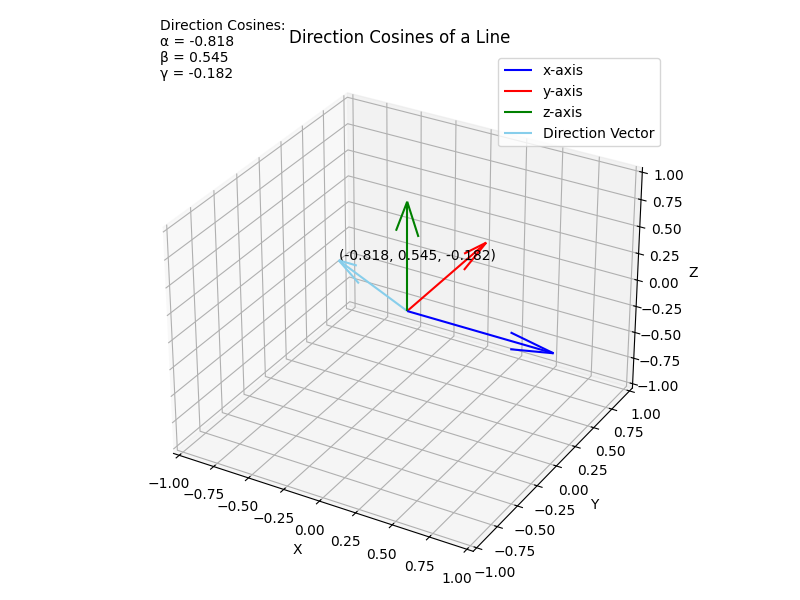
\includegraphics[width=0.5\linewidth]{figs/plot.png}
        \caption{plot}
        \label{fig:placeholder}
    \end{figure}
\end{frame}


\end{document}